\chapter{HPL-AI算法分析与实现}

\label{HPL-AI算法分析与实现}

\section{HPL-AI基准规则}

根据HPL-AI的主页\cite{dongarrahpl},我们归纳了这一新基准的主要思想,主要包括以下两点:

\begin{enumerate}
    \item 对矩阵进行混合精度分解,然后计算较低精度分解下得到的近似解。
    \item 使用前一步得到的解作为预条件(preconditioner),使用 64 位精度的迭代方法(如 GMRES)迭代,最终得到与 64 位精度 LU 分解相当的精确度。
\end{enumerate}

\subsection{矩阵构造}

基准的实现应当参照 HPL,但需要修改矩阵生成器:应当构造一个非对称的对角优势(diagonally dominant)矩阵,可以保证用直接法或迭代法解线性代数方程组的稳定性和收敛性。

\subsection{混合精度}

分解过程可以使用混合精度,例如:panel 分解和三角矩阵求解可以用 32 位精度完成,舒尔补充过程(Schur complement,即$A_{2,2} \leftarrow A_{2,2} - A_{2,1} \times A_{1,1}^{-1} \times A_{1,2}$ 形式的矩阵乘法)可以用 32 位累加的 16 位精度来计算。

为了在所有计算机上实现一致的性能标准,在基准测试过程中求解低精度方程组时使用的算法必须在数学上等价于 LU 因式分解,且所需的浮点操作数(即使不需要双精度运算)必须是 $\frac{2}{3} n^3 + \frac{3}{2} n^2$(LU 因式分解需要 $\frac{2}{3} n^3 - \frac{1}{2} n^2$,$2n^2$ 用于随后的后向和正向求解)。

同时,HPL-AI允许在浮点格式范围内对结果进行平衡缩放,但所需的时间必须包含在求解时间中。

\subsection{误差与限制}

HPL-AI的误差由此式确定:
$$
    \frac{\Vert Ax-b\Vert_{\infty}}{\Vert A\Vert_{\infty} \Vert x\Vert_{\infty} + \Vert b\Vert_{\infty}} \times (n \times \epsilon)^{-1}
$$
其中,$n$ 是输入矩阵的大小;$\epsilon$ 是 64 位浮点算术中的机器精度,在 IEEE 标准下有 $\epsilon=2^{−53}\approx 1.1\times 10^{-16}$。

HPL-AI的规则对 $n$ 没有限制,但数值迭代至多不能超过50轮,且其得到的最终误差必须小于 $16$。

\subsection{提交结果}

HPL-AI的计算效率基于计算系统求解问题的时间总和:较低精度矩阵分解过程、(可能的)防止溢出的平衡放缩过程、执行 GMRES 或使用 LU 因子作为预条件的使用 64 位浮点运算的其他迭代过程。在计算效率时,用$\frac{2}{3} n^3 + \frac{3}{2} n^2$除以总的解算时间,得到每秒的运算速率。

作为提交结果的一部分,提交者被希望提供提交中使用的算法的详细说明。

\section{矩阵生成器}

\autoref{matA}给出我们构造的矩阵在数学上的描述,其中$\alpha,\beta$为矩阵的构造参数,可通过\cite{2021Matrices}中的方法选取。此处我们我们设置条件数$\kappa=100$,比例系数$\rho=0.5$,则有$\beta=2.50/N,\alpha=\rho\beta=1.25/N$。同时,我们也使用了来自\cite{2021Matrices}的系数$\psi=f_{\max}/2=65504/2$对矩阵进行缩放,使得该矩阵可以在FP16精度下被安全分解。

\begin{equation}
    \left(A\left(\alpha,\beta\right)\right)_{i,j}=\begin{cases}
        -\alpha+\left(j-1\right)\alpha\beta & \text{if } i>j \\
        1+\left(i-1\right)\alpha\beta       & \text{if } i=j \\
        -\beta+\left(i-1\right)\alpha\beta  & \text{if } i<j \\
    \end{cases}\label{matA}
\end{equation}

根据\cite{2021Matrices}中的证明,$\psi A\left(\alpha,\beta\right)$可以在$O(n^2)$的浮点操作内构造,且不需要选取主元即可稳定LU分解,符合HPL-AI基准要求.

\section{LU分解算法}

我们基于 HPL 软件包的实现,使用 LU 分解方法求解线性方程组。LU 分解存在三种方法,right-looking,left-looking 和 crout-looking,此处采用的是更容易被并行化的 right-looking 的分解方法\cite{2013Correcting}。\autoref{equ:right-looking} 给出right-looking LU分解的数学描述。

\begin{equation}
    \label{equ:right-looking}
    \begin{bmatrix}
        A_{1,1} & A_{1,2} \\
        A_{2,1} & A_{2,2}
    \end{bmatrix}
    =
    \begin{bmatrix}
        L_{1,1} & 0       \\
        L_{2,1} & L_{2,2}
    \end{bmatrix}
    \begin{bmatrix}
        U_{1,1} & U_{1,2} \\
        0       & U_{2,2}
    \end{bmatrix}
\end{equation}

以下是具体分解顺序:

\begin{wrapfigure}{r}{0.3\linewidth}
    \centering
    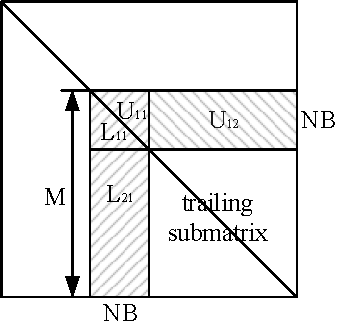
\includegraphics[width=0.3\textwidth]{image/chap02/LU}
    \caption{对输入矩阵 A 进行 LU 分解的示意图}
    \label{对输入矩阵 A 进行 LU 分解的示意图}
\end{wrapfigure}

\begin{enumerate}
    \item $A_{1,1} \leftarrow L_{1,1} U_{1,1},A_{2,1} \leftarrow L_{2,1}U_{1,1}$
    \item $A_{1,2} \leftarrow L_{1,1} U_{1,2}$
    \item $A_{2,2} \leftarrow A_{2,2} - L_{2,1}U_{1,2}$
    \item $A_{2,2} \leftarrow L_{2,2}U_{2,2}$
\end{enumerate}

\autoref{对输入矩阵 A 进行 LU 分解的示意图} 给出了对输入矩阵进行分解的示意图。分解过程中,每次循环迭代分解一个 $M\times\mathit{NB}$ 的矩阵,这个被分解的 $\mathit{NB}$ 列矩阵称之为 panel,$\mathit{NB}$ 是算法的输入参数,在输入文件 \lstinline{HPL.dat} 中指定。第一步是对 $\mathit{NB}$ 列、$M$ 行的矩阵进行分解,得到 $L_{1,1}$、$U_{1,1}$ 和 $L_{2,1}$,这一步称之为 panel 分解(panel factorization),在分解过程中,同时会执行 panel 内的选主元操作,并将结果进行保存;第二步进行三角矩阵求解(trsm),得到 $U_{1,2}$;第三步
    是对 $(M-\mathit{NB}) \times (M-\mathit{NB})$ 的剩余子矩阵(trailing submatrix)进行更新(gemm),得到待分解的 $L_{2,2}U_{2,2}$。

    通过如上三个步骤,成功把输入矩阵求解的问题转换成剩余子矩阵 $\leftarrow L_{2,2}U_{2,2}$ 的求解问题。于是,后续迭代只需要对重复对剩余子矩阵应用上述三个步骤,即可完成对整个问题的求解。

    \subsection{LU分解的并行化}
    \label{LU分解的并行化}

    \begin{wrapfigure}{r}{0.5\linewidth}
        \centering
        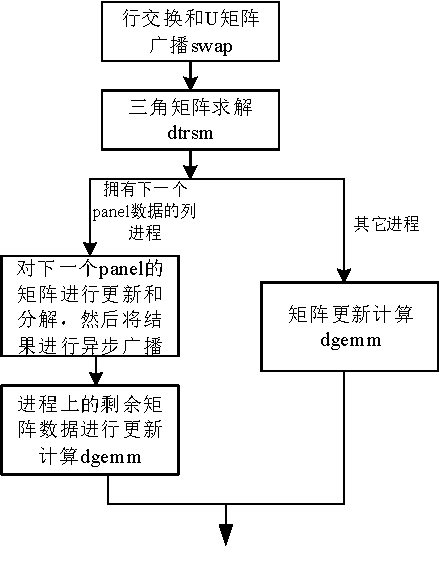
\includegraphics[width=0.5\textwidth]{image/chap02/PLU}
        \caption{并行LU分解的基本步骤图}
        \label{并行LU分解的基本步骤图}
    \end{wrapfigure}

    我们沿用了来自HPL的并行LU分解算法,\autoref{并行LU分解的基本步骤图}给出了该算法的基本步骤图。我们将所有参与计算的$\mathit{np}$个进程组织成一个二维的$P\times Q$进程网格,以$\mathit{NB}\times\mathit{NB}$为单位block-cyclic的方式均匀映射到输入矩阵$A$;$P,Q,\mathit{NB}$等是算法的输入参数,进程排列可选row-major和column-major两种方式。Panel分解完成后,panel所在的列进程将分解后的结果进行广播。然后,在剩余子矩阵中进行行交换,并广播U矩阵,这一步称之为swap。随后,在每个进程上进行trsm的计算过程。最后一步,对剩余子矩阵进行矩阵更新操作。

    \autoref{输入矩阵在进程间的分配图}给出了row-major映射下$P=2,Q=4$时,进程分布和输入矩阵在进程间的数据分配图,阴影部分数据为当前panel,其所在的列进程为5和1号进程,panel广播操作是5号进程将其所有的当前panel的分解结果广播给其它的行进程,即6、7和4号进程;同时,1号进程将其所有的panel分解结果广播给予其在同一行的进程,即2、3和0号进程。U矩阵广播操作是6号进程将其所有的U矩阵广播给予其在同一列上的2号进程,同时,7和4号进程也将其所有的U广播给予其在同一列的进程。

    \begin{wrapfigure}{r}{0.3\linewidth}
        \centering
        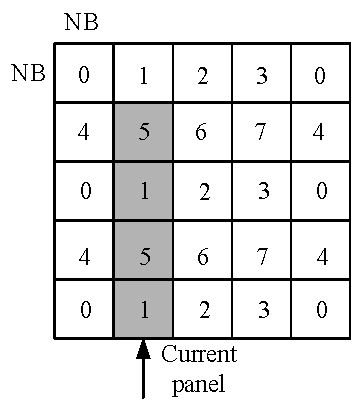
\includegraphics[width=0.3\textwidth]{image/chap02/LUP}
        \caption{输入矩阵在进程间的分配图}
        \label{输入矩阵在进程间的分配图}
    \end{wrapfigure}

    注意到Panel广播和矩阵更新没有依赖关系,可以并发执行以隐藏广播开销,这也是来自HPL中的一种通信优化方法,被称作Lookahead。拥有下一个Panel的列进程步骤是:首先,对下一个panel的矩阵数据进行更新计算,然后,对更新结果进行panel分解,并将分解结果在行向进行异步广播,最后,更新进程上的剩余子矩阵。同时,所有的其它进程进行当前剩余子矩阵的更新计算。这样就实现了下一个panel的广播和当前剩余子矩阵更新计算的重叠。

    \subsection{Panel分解}

    Panel分解是整个LU分解计算的关键步骤\cite{2013Correcting},拥有当前panel数据的所有列进程参与分解计算。三种LU分解算法均可用于panel分解,并可由输入参数中的recursive panel fact参数指定:left-looking、right-looking和crout-looking。这三种算法都是以递归方式实现的,递归分解的粒度根据输入参数中的$\mathit{NBMIN}$和$\mathit{NDIV}$两个参数控制:$\mathit{NBMIN}$是递归算法的停止条件,指定了进行分解的最少列数;$\mathit{NDIV}$是用于确定每个panel被划分成子panel的数目。当前Panel的$\mathit{NB}$列矩阵每次以$\mathit{NDIV}$份进行递归的列划分,直到最小列$\mathit{NBMIN}$。

    接下来我们以$\mathit{NB}=256,\mathit{NBMIN}=8,\mathit{NDIV}=4$的参数为例,对三种panel分解算法流程进行描述。256列的panel首先被分成4个subpanel,每个subpanel是64列的矩阵,在后面的描述中以subp 1, subp 2等代替。由于$64>\mathit{NBMIN}$,因此,每个64列的矩阵继续被分成4个subpanel,每个subpanel是16列。由于$16/\mathit{NDIVs}=4<\mathit{NBMIN}$,所以无法再对16列的subpanel进行划分,得到的最小subpanel的列数为16。最小的subpanel在后面的描述中分别以subp a, subp b等代替。

    \subsubsection{left-looking}

    \begin{wrapfigure}{r}{0.5\linewidth}
        \centering
        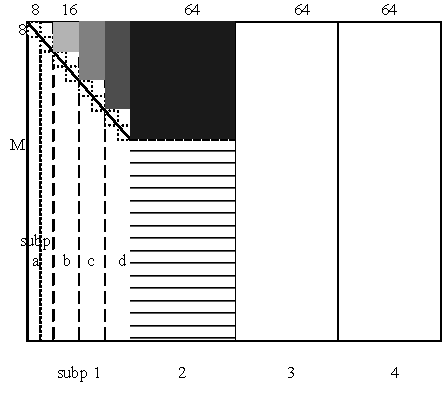
\includegraphics[width=0.5\textwidth]{image/chap02/left-looking}
        \caption{left-looking分解算法}
        \label{left-looking分解算法}
    \end{wrapfigure}

    \autoref{left-looking分解算法}给出left-looking分解算法图示。首先,对subp a进行分解;然后,进行dtrsm计算,得到subp b中的U矩阵(阴影部分);随后,利用subp a中的矩阵和U矩阵更新subp 中的trailing submatrix;最后,对更新后的subp b的trailing submatrix进行分解计算,这样就完成了subp b的分解计算。按照同样的步骤完成对subp c和subp d的计算工作。这样,就完成了对subp 1的分解计算。接下来,进行trsm计算得到subp 2的U矩阵,并对subp 2的trailing submatrix进行更新计算。随后,对subp 2的分解计算步骤和subp 1的分解步骤完全相同。按照这种递归方法,完成对subp 3和subp 4的分解计算,就完成了对整个panel的分解计算。

    \subsubsection{crout-looking}

    \begin{wrapfigure}{r}{0.5\linewidth}
        \centering
        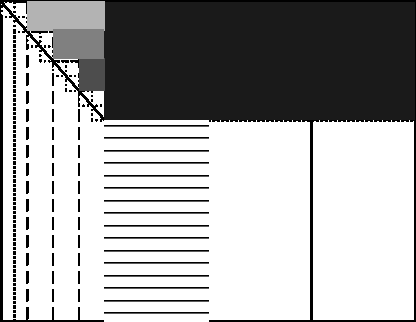
\includegraphics[width=0.5\textwidth]{image/chap02/crout-looking}
        \caption{crout-looking分解算法}
        \label{crout-looking分解算法}
    \end{wrapfigure}

    \autoref{crout-looking分解算法}给出crout-looking分解算法图示。首先,对subp a进行分解;然后,进行trsm计算,得到subp 1中$16\times48$的U矩阵(subp 1中最上层的阴影部分);随后,对subp b中的$(M-16)\times16$的trailing submatrx进行更新;最后,对subp b进行分解计算,这样就完成了subp b的分解计算。按照同样的步骤,完成subp c和subp d的分解计算。接下来,进行trsm计算得到整个panel的一个$64\times192$的U矩阵,并对subp 2的$(M-64)\times64$的trailing submatrix进行更新计算。以此递归方式完成对完成了对整个panel的分解计算。

    \subsubsection{right-looking}

    \begin{wrapfigure}{r}{0.5\linewidth}
        \centering
        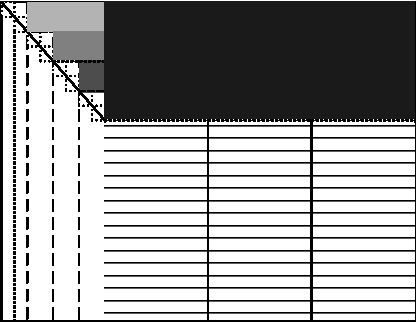
\includegraphics[width=0.5\textwidth]{image/chap02/right-looking}
        \caption{right-looking分解算法}
        \label{right-looking分解算法}
    \end{wrapfigure}

    \autoref{right-looking分解算法}给出right-looking分解算法图示。首先,对subp a进行分解;然后,进行trsm计算,得到subp 1中$16\times48$的U矩阵(subp 1中最上层的阴影部分);随后,对subp 1中的$(M-16)\times48$的trailing submatrx进行更新;最后,对subp b进行分解计算,这样就完成了subp b的分解计算。按照同样的步骤,完成subp c和subp d的分解计算。接下来,进行trsm计算,得到剩余panel的一个$64\times192$的U矩阵,并对整个panel的$(M-64)×192$的trailing submatrix进行更新计算。以此递归方式完成对完成了对整个panel的分解计算。

    \section{数值迭代算法}

    在问题求解的IR阶段,我们参照了来自HPL-AI主页实现的GMRES算法(Generalized Minimal Residual,广义最小残差算法)\cite{1986GMRES},并将其扩展到与HPL相同进程分布的MPI实现,尽可能减少数据重组和额外通信。GMRES是一种求解形如$Ax=b$线性形式方程的高效迭代算法。利用Arnoldi迭代法,将线性方程转化为一个线性最小二乘法的问题,再最小化这个残余量矢量,从而通过初始解$x_0$求出$x$在Krylov子空间的近似解。

    \subsection{Householder变换}

    传统GMRES使用Arnoldi算法将矩阵转换为Hessenberg矩阵,并利用Givens旋转法对Hessenberg矩阵进行处理。虽然这是最经典的方法,但是稳定性不够高,在实验中我们发现其容易使得GMRES收敛慢。

    因此,我们使用了Householder变换代替Arnoldi算法的格拉姆-施密特正交化过程,通过额外引入少量计算得到更加稳定的结果。\cite{1988Implementation}给出了使用Householder变换的GMRES算法的完整流程及数学证明,\autoref{使用Householder变换的GMRES算法}是该算法的伪代码。

    \begin{algorithm}[h]
        \KwIn{初始解$x_0$,容错值$\mathit{TOL}$,迭代轮数$\mathit{MAXIT}$}
        初始化:$L_1=(1),U_1=(u_1),r_0=b-Ax_0$\;
        确定$P_1$使得$P_1r_0=\pm\lVert r_0\rVert_2e_1$\;
        \ForEach{$m=1,2,\dots,\mathit{MAXIT}$}{
        计算$v\equiv \lbrace I-2U_mL_m^{-1}U_m^T\rbrace A \lbrace I-2U_m(L_m^T)^{-1}U_m^T\rbrace e_m$\;
        \If{$v^{(m+1)}=\dots=v^{(n)}=0$不满足}{
        计算$P_{m+1}=I-2u_{m+1}u_{m+1}$,其中$u_{m+1}$的前$m$个组分为零,这样$P_{m+1}v$在第$(m+1)st$之后具有零组分\;
        更新$v\leftarrow P_{m+1}v$\;
        }
        \If{$m>1$}{更新$v\leftarrow J_{m-1}\dots J_1v$}
        \If{$v^{(m+1)}\neq0$}{
            确定用于组分$m,m+1$的$J_m$,使得$\left(J_mv\right)^{\left(m+1\right)}=0$\;
            更新$v\leftarrow J_mv,w\leftarrow J_mw$\;
        }
        设置$R_m=\begin{cases}
                \left(v\right)         & \text{if } m=1 \\
                \left(R_{m-1},v\right) & \text{if } m>1
            \end{cases}$\;
        \If{$m<\mathit{MAXIT}$且$\lvert w^{(m+1)}\rvert>\mathit{TOL}$}{
            计算$L_{m+1}=\begin{bmatrix}
                    L_m           & 0 \\
                    2u_{m+1}^TU_m & 1
                \end{bmatrix}$;
            计算$U_{m+1}=\begin{bmatrix}U_m & u_{m+1}\end{bmatrix}$\;
        }
        \Else{
            求解$R_m$的上三角矩阵作为系数矩阵、$w$作为右手列的线性方程组,得到使得$\lVert 2-R_my\rVert_2$最小的$y_m$\;
            更新$x_0\leftarrow x_0+\lbrace I-2U_m\left(L_m^T\right)^{-1}U_m^T\rbrace\left(e_1,\dots,e_m\right)y_m$\;
            \If{$\lvert w^{(m+1)}\rvert>\mathit{TOL}$}{
                以当前的$x_0$作为输入,重新递归进行本算法\;
            }
            退出算法,返回结果$x_0$\;
        }
        }
        \caption{使用Householder变换的GMRES算法}
        \label{使用Householder变换的GMRES算法}
    \end{algorithm}

    值得注意的是,$\mathit{TOL}$是不同于HPL-AI算法的误差值的一个参数。

    \subsection{运行策略}
    \label{运行策略}

    GMRES 的主要缺点是:每次迭代所需的时间复杂度和空间复杂度会随着迭代次数的上升而增加。因此,除非(幸运地)很快就能够收敛,计算代价将迅速变得令人望而却步。

    克服这种限制的通常方法是重启迭代。在选定的迭代次数$m$之后,清除累积数据,中间结果被用作下一次迭代的初始数据;重复此过程,直到自身的误差值$<\mathit{TOL}$。不幸的是,$m$的选取没有明确的规则,这是一个经验问题。$m$过大,算法的时间和空间开销会超过起来来的收益;$m$过小,难以得到足够收敛的结果。

    与HPL-AI参考实现相同,我们使用$m=50$,并将GMRES自身的容错值设置成$\mathit{TOL}=\epsilon/2.0/(n/4.0)$。其中,$n$ 是输入矩阵的大小;$\epsilon$ 是 64 位浮点算术中的机器精度,在 IEEE 标准下有 $\epsilon=2^{−53}\approx 1.1\times 10^{-16}$。

    与参考实现不同的是,为减少运行时的开销,我们并没有在每轮迭代之后检查HPL-AI自身的误差。当然,从理论上来说,此处的参数选择有可能导致返回的结果误差超过HPL-AI的限制(例如当$N/\mathit{NB}$的比值不合理,导致浮点数的累加误差增大)。但根据我们的实验结果,在$N\sim 10^{5}$的时候,我们的实现可以在大部分情况下得到收敛的结果,并相对于LU分解过程有极小的开销。

此外我们甚至发现,在ARM64环境下链接到 openblas@0.3.8 及以下版本并开启OpenMP支持时,因其存在的多线程race的bug,HPL会概率返回错误的运行结果\footnote{详见\url{https://github.com/wu-kan/HPL-AI/issues/1},解决方法见\autoref{软件依赖}};而此时HPL-AI使用了数值迭代,反而可以返回正确的值。这说明我们的GMRES实现及其参数选择有很高的鲁棒性。

\section{面临的挑战}

结合上述分析,要针对一个计算系统实现高性能的HPL-AI基准,需要面临如下挑战,这也是我们在\autoref{面向国产异构处理器的移植工作}中致力于解决的目标。


\subsection{针对硬件的混合精度算法设计}

现代的硬件平台通常针对新兴的AI应用提供了包括FP16、BF16在内的多种计算精度支持\footnote{\url{https://nhigham.com/2018/12/03/half-precision-arithmetic-fp16-versus-bfloat16/}},他们的性能通常远优秀于传统HPC应用中使用的FP64、FP32。

因此,需要结合具体硬件规格,在不同计算阶段选用不同的精度和计算设备。例如,可以在panel分解和三角矩阵求解中使用FP32在CPU完成,在矩阵乘法更新剩余子矩阵过程中使用FP16/BF16/TF32在异构处理器上完成。同时,也需要考虑引入额外的放缩过程/数值迭代过程,减少/恢复计算过程中的精度损失。

\subsection{异构计算中的负载均衡问题}

目前主流的超算系统均为异构系统,在通用CPU之外同时搭载高性能的异构处理器用于处理专用问题。这类系统通常需要由CPU将任务传输到异构处理器上,并且等待异构处理器将任务完成。

因此,由此引入的任务传输开销及负载问题仍然是需要考虑的。例如,可以使用CPU负载部分任务,在减少异构处理器的负载同时掩盖CPU和异构处理器的传输开销。

\subsection{高性能的BLAS和MPI过程实现}

HPL/HPL-AI中包含了大量线性代数过程调用,其计算的绝大部分是gemm和trsm两个关键步骤,其性能取决于BLAS库(Basic Linear Algebra Subprograms)的性能\cite{endo2010linpack}。根据实验中的经验,本质为矩阵乘法的剩余矩阵更新占据了主要计算时间的80\%以上。此外,计算系统中进程间的通信问题同样会极大影响整体运算的效率,而HPL/HPL-AI中的通信过程一般通过MPI标准实现。

因此,针对计算系统实现的HPL-AI基准应当包含高效的BLAS和MPI实现,并且应当针对硬件架构和计算过程中的各种问题规模进行调优,以充分利用整个系统的算力。
